\documentclass{beamer}
\usetheme{Warsaw}

\usepackage[utf8]{inputenc}
\usepackage{fancybox}
\usepackage{multimedia} 
\usepackage{subfig}
\usepackage{amsmath}
\usepackage{hyperref}
\usepackage[all]{xy}
\begin{document}


\title[Angewandte Mathematik] % (optional, only for long titles)
{Angewandte Mathematik
\\
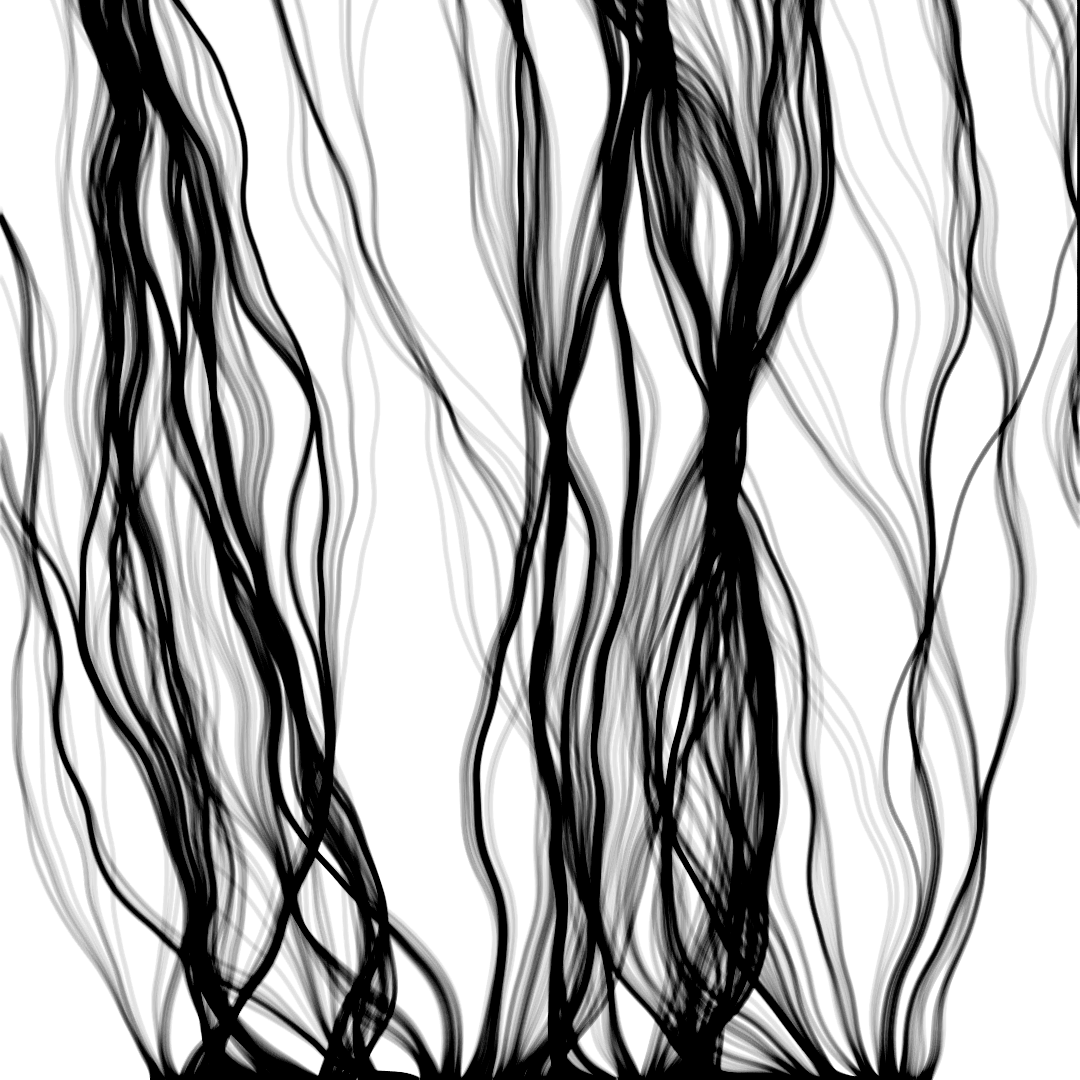
\includegraphics[scale=0.15]{images/cover}
}
\subtitle{}
\author[Dr. Johannes Riesterer] % (optional, for multiple authors)
{Dr.  rer. nat. Johannes Riesterer}

\date[KPT 2004] % (optional)
{}

\subject{Angewandte Mathematik}

\frame{\titlepage}

\begin{frame}
    \frametitle{Angewandte Mathematik}
\framesubtitle{}
    \begin{block}{Was ist Angewandte Mathematik?}
\begin{itemize}
\pause \item Algorithmen zum Lösen von Problemen.
\pause \item Abschätzungen, wie gut und genau die Algorithmen funktionieren.
\pause \item Mathematische Grundlagen, auf denen Algorithmen und Abschätzungen basieren. 
\pause \item Softwaretechnische Aspekte in Bezug auf  Implementierung der Algorithmen.
\end{itemize}
\end{block}
 \end{frame}

\begin{frame}
    \frametitle{Angewandte Mathematik}
\framesubtitle{}
    \begin{block}{Kann jeder Mathematik lernen?}
 Lebenslauf einer von Emmy Noether, einer der bedeutendsten Mathematikerinnen aller Zeiten eingehen  (Auszug aus Wikipedia):
... Sie zeigte in mathematischer Richtung keine besondere Frühreife, sondern hatte in ihrer Jugend Interesse an Musik und Tanzen. Sie besuchte die Städtische Höhere Töchterschule – das heutige Marie-Therese-Gymnasium – in der Schillerstraße in Erlangen. Mathematik wurde dort nicht intensiv gelehrt. Im April 1900 legte sie die Staatsprüfung zur Lehrerin der englischen und französischen Sprache an Mädchenschulen in Ansbach ab. 1903 holte sie in Nürnberg die externe Abiturprüfung am Königlichen Realgymnasium – dem heutigen Willstätter-Gymnasium – nach. 
\end{block}
 \end{frame}


\begin{frame}
    \frametitle{Angewandte Mathematik}
\framesubtitle{}
    \begin{block}{Kann jeder Mathematik lernen?}
\begin{itemize}
\pause \item Oft ist Mathematik ein Motivationsproblem.
\pause \item Starten mit  Beispielen, die motivieren sollen, wozu der Stoff gut ist.
\pause \item Unterfüttern Beispiele mit  Softwarecode. 
\pause \item Rechnen Übungsaufgaben.
\end{itemize}
\end{block}

 \end{frame}


\begin{frame}
    \frametitle{Angewandte Mathematik}
\framesubtitle{}
    \begin{block}{Stoff}
\begin{itemize}
\pause \item Mehrdimensionale Differentialrechnung $->$ Backpropagation zum Trainieren Neuronaler Netze.
\pause \item Mehrdimensionale Integralrechnung $->$ Signalanalyse mit FFT, Abtast-Theorem von Shanon, Bildverarbeitung
\pause \item Gewöhnliche Integralgleichungen (ODE) $->$ Vorhersage von zeitlich abhängigen, deterministischen Vorgängen.
\pause \item Partielle Integralgleichungen $->$ Vorhersage von zeitlich und räumlich abhängigen, deterministischen Vorgängen.
\end{itemize}
\end{block}

 \end{frame}


\begin{frame}
    \frametitle{Mehrdimensionale Differentialrechnung}
\framesubtitle{Motivation}
    \begin{block}{Neuroanles Netz}
\begin{figure}[htp]
    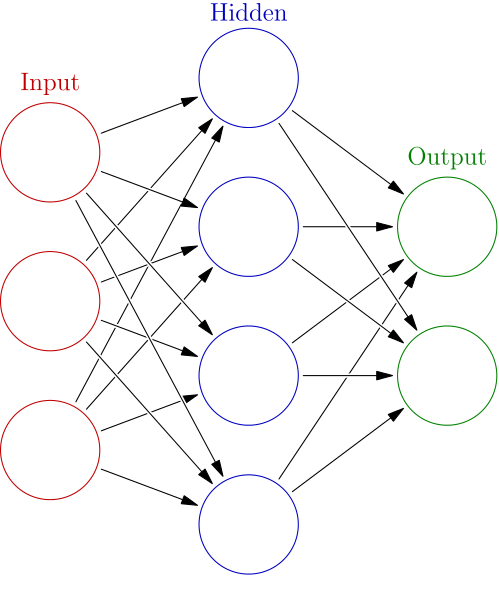
\includegraphics[width=0.15\textwidth]{images/499px-Colored_neural_network}
      \caption{Quelle: Wikipedia}
\end{figure}
\end{block}
    \begin{block}{Motivation}
\begin{figure}[htp]
    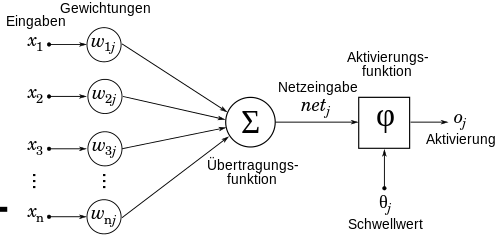
\includegraphics[width=0.35\textwidth]{images/500px-NeuronModel_deutsch}
      \caption{Quelle: Wikipedia}
\end{figure}
\end{block}
 \end{frame}

\begin{frame}
    \frametitle{Mehrdimensionale Differentialrechnung}
\framesubtitle{Motivation}
    \begin{block}{Neuronales Netz}
Ein  neuronales Netz lässt sich als Funktion $f(\omega, x)$ mit Gewichten $\omega$ und Input $x$ auffassen.
Diese  ist aus einzelnen, einfachen Teilen zusammengesetzt.
\end{block}

\uncover<2->
{
    \begin{block}{Neuronales Netz trainieren}
Gegeben Datensatz $D$. Finde Gewichte Omega, so dass Lossfunktion
\begin{align*}
L_D  : \Omega \subset \mathbb{R}^n \to \mathbb{R} 
\end{align*}
minimal wird. Zum Beispiel $L_D(\omega) := \sum_{(x,y) \in D} (f(\omega, x) - y)^2$.
\end{block}
}
 \end{frame}


\begin{frame}
    \frametitle{Mehrdimensionale Differentialrechnung}
\framesubtitle{Motivation}
    \begin{block}{Backpropagation}
Standard verfahren ist das sogenannte Backpropagation-Verfahren.
Im Wesentlichen Ableitung hochdimensionaler, zusammengesetzter Funktionen berechnen.
\end{block}

\begin{figure}[htp]
    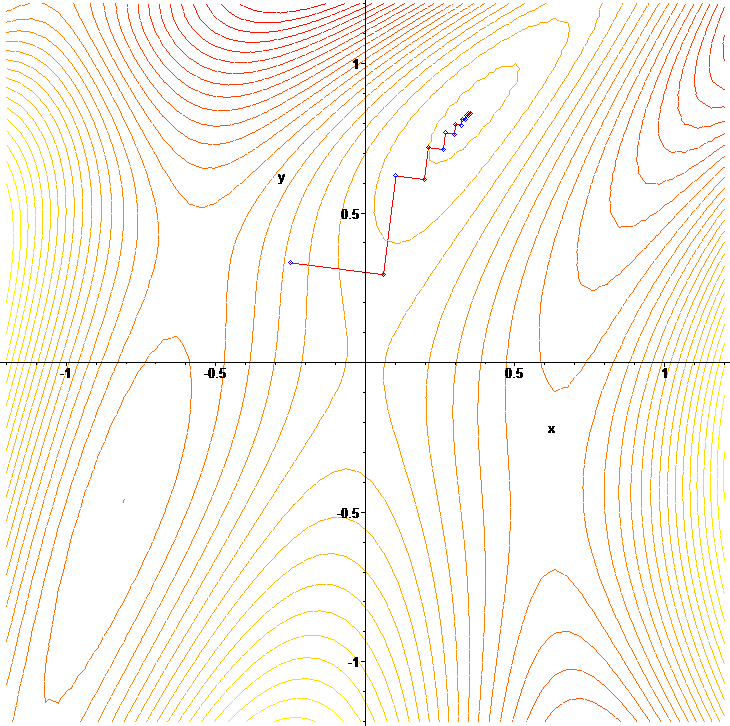
\includegraphics[width=0.35\textwidth]{images/Gradient_ascent}
      \caption{Quelle: Wikipedia}
\end{figure}
 \end{frame}


\begin{frame}
    \frametitle{Mehrdimensionale Differentialrechnung}
\framesubtitle{Vorwissen über eindimensionale  Funktionen}
    \begin{block}{Differenzierbarkeit reeller Funktionen}
Eine reelle Funktion $f : (a, b) \to \mathbb{R}$  heißt differenzierbar in $x \in (a,b)$, falls der Grenzwert $\lim_{h \to 0}  \frac{f(x +h) - f(x)}  {h}$ existiert. In diesem Fall heißt dieser Grenzwert die Ableitung (Steigung) von $f$ in $x$ und wird mit $f' (x)$ bezeichnet.
\end{block}
\begin{figure}[H]
      \centering
    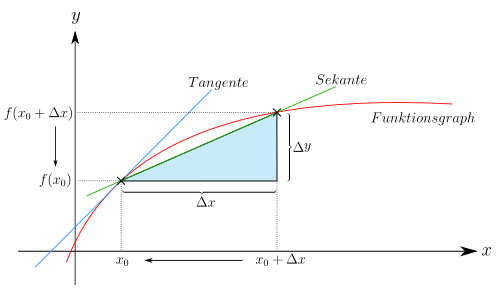
\includegraphics[width=0.5\textwidth]{images/Differencial_quotient_of_a_function}
      \caption{Quelle: Wikipedia: https://de.wikipedia.org/wiki/Datei:Differencial\_quotient\_of\_a\_function.svg}
\end{figure}
 \end{frame}

\begin{frame}
    \frametitle{Mehrdimensionale Differentialrechnung}
\framesubtitle{Vorwissen über eindimensionale  Funktionen}
    \begin{block}{Mittelwertsatz einer Veränderlichen}
Sei $f : [a,b] \to \mathbb{R}$ stetig und differenzierbar für alle $x \in (a,b)$. Dann gibt es $\xi \in (a,b)$ mit
$f'(\xi) = \frac{f(b) - f(a)} { b-a}$.
\end{block}
\begin{figure}[H]
      \centering
    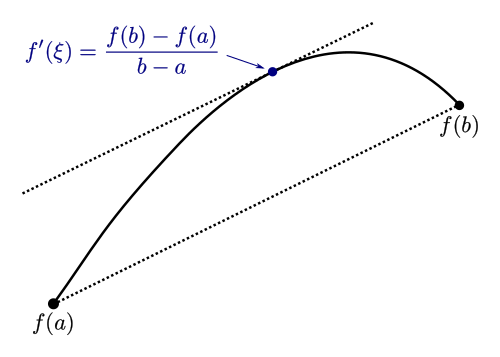
\includegraphics[width=0.5\textwidth]{images/Mittelwertsatz3.png}
      \caption{Quelle: Wikipedia: https://commons.wikimedia.org/wiki/File:Mittelwertsatz3.svg}
\end{figure}
 \end{frame}


\begin{frame}
    \frametitle{Mehrdimensionale Differentialrechnung}
\framesubtitle{Vorwissen über eindimensionale  Funktionen}
    \begin{block}{Taylorapproximation einer Veränderlichen}
Jede  reelle Funktion $f$, deren $p+1$-ten Ableitungen existieren und stetig sind lässt sich mit Hilfe der Taylorreihe  
\begin{align*}
&f(x) = f(a) + \frac{1}{2!} f^{'} (x-a) +   \frac{1}{3!} f^{''}(a) (x-a)^2 + \cdots  \\
& +  \frac{1}{p!} f^{(p)}(a) (x-a)^{p-1} +  R_{p+1}(x,a) 
\end{align*}
und dem Restglied  $R_p(x,a) :=   \frac{1}{(p+1)!} f^{(p+1)}(\xi) (x-a)^{p} $ mit einem $\xi \in (x,a)$ darstellen.
\end{block}

 \end{frame}

\begin{frame}
    \frametitle{Mehrdimensionale Differentialrechnung}
\framesubtitle{Vorwissen über eindimensionale  Funktionen}
    \begin{block}{Cauchy-Schwarzsche Ungleichung}
 Für zwei Vektoren $v,w \in \mathbb{R}^n$ gilt: 
\begin{align*}
\frac{\langle v, w \rangle}{||v|| \cdot ||w||} = \cos(\varphi) 
\end{align*}
wobei $\varphi$ der Innenwinkel zwischen $v$ und $w$ ist.
\end{block}

 \end{frame}


\begin{frame}
    \frametitle{Mehrdimensionale Differentialrechnung}
\framesubtitle{Vorwissen über eindimensionale  Funktionen}
    \begin{block}{Äquivalenz von Normen}
 Die Normen $||v||: = \sqrt{\sum_{i = 1}^n v_i^2}$ und $||v||_{\infty}:= \max \{ v_1, \cdots, v_n \} $ sind Äquivalent. Sie lassen sich  mit Konstanten $k_1 ||v|| < ||v||_{\infty}  < k_2  ||v|| $ gegeneinander abschätzen.
\end{block}

 \end{frame}

\begin{frame}
    \frametitle{Mehrdimensionale Differentialrechnung}
\framesubtitle{Vorwissen über eindimensionale  Funktionen}
    \begin{block}{Symmetrische Matrizen}
 Für eine symmetrische Matrix $A \in \mathbb{R}^{n \times n}$ ist Äquivalent:
\begin{itemize}
\item $A$ hat positive Eigenwerte.
\item Für alle $v \in \mathbb{R}^n \neq 0$ gilt  $v^TA v > 0 $.
\item alle Unterdeterminanten sind positiv. Speziell für $n=2$ und $A = \begin{pmatrix} a & b \\ b & d\end{pmatrix}$ bedeutet dies
$a >0$ und $ad -b^2 >0$. 
\end{itemize}
\end{block}

 \end{frame}


\begin{frame}
    \frametitle{Mehrdimensionale Differentialrechnung}
\framesubtitle{Limes}
    \begin{block}{Konvergenz}
Eine Folge $(a_n)$ in $\mathbb{R}^n$ heißt konvergent gegen den Grenzwert $a \in \mathbb{R}^n$, wenn gilt:
\begin{align*}
\forall {\varepsilon > 0} \ \exists \ N \in \mathbb{N} \; \forall \ n > N: \; d(a, a_n) < \varepsilon\,
\end{align*}
in Worten: Es gibt für jedes beliebige (noch so kleine) $\varepsilon$ einen Index $N$ derart, dass für alle Indizes $n > N$, alle weiteren Folgenglieder, gilt: der Abstand $d(a, a_n)$ ist kleiner als $\varepsilon$.
\end{block}
\begin{figure}[H]
      \centering
    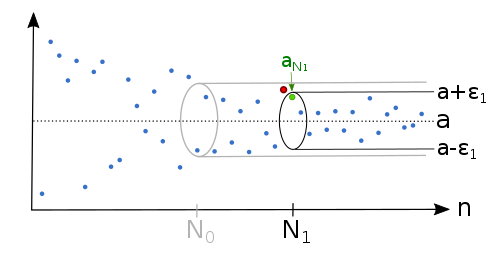
\includegraphics[width=0.4\textwidth]{images/500px-Epsilonschlauch_klein}
      \caption{Quelle: Wikipedia: https://commons.wikimedia.org/wiki/File:Epsilonschlauch\_klein.svg}
\end{figure}

 \end{frame}

\begin{frame}
    \frametitle{Mehrdimensionale Differentialrechnung}
\framesubtitle{Limes}
    \begin{block}{Konvergenz}
Sei $f :X \subset \mathbb{R}^n \to \mathbb{R}^m$ eine  Funktion und $a \in X$. Wir nennen $L_a \in \mathbb{R}^m$ Grenzwert von $f$ bezüglich der Annäherung von $x$ an $a$, falls für jede  konvergente Folge $x_n \to a$  die Folge $f(x_n)$ nach $L_a$ konvergiert.  In diesem Fall bezeichnen wir
\begin{align*}
\lim_{x \to a} f(x) = L_a \;.
\end{align*}
Dies ist gleichbedeutend damit, dass für jedes $\epsilon > 0$ ein $\delta > 0$ existiert, so dass
$d(f(x) ,L_a) < \epsilon$ gilt für jedes $x$ mit $d(x, a) < \delta$.
\end{block}


 \end{frame}


\begin{frame}
    \frametitle{Mehrdimensionale Differentialrechnung}
\framesubtitle{Limes}

\begin{figure}[H]
      \centering
    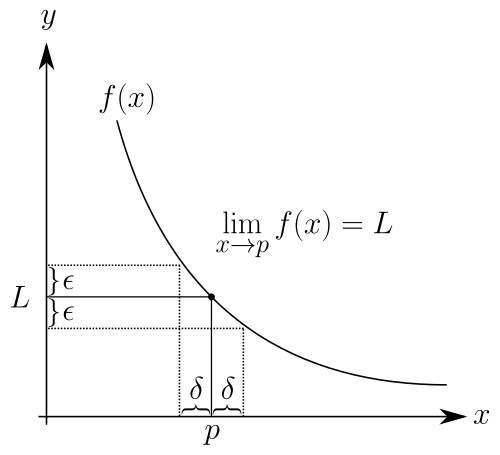
\includegraphics[width=0.3\textwidth]{images/500px-Limes_Definition_Vektorgrafik}
      \caption{Quelle: Wikipedia: https://de.wikipedia.org/wiki/Datei:Limes\_Definition\_Vektorgrafik.svg}
    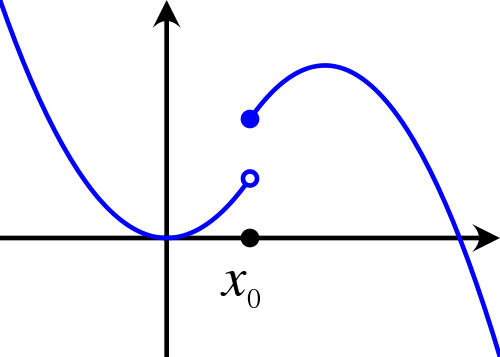
\includegraphics[width=0.3\textwidth]{images/500px-Upper_semi}
      \caption{Quelle: Wikipedia: https://commons.wikimedia.org/wiki/File:Upper\_semi.svg}
\end{figure}

 \end{frame}



\begin{frame}
    \frametitle{Mehrdimensionale Differentialrechnung}
\framesubtitle{Limes}
    \begin{block}{Stetigkeit}
Eine reellwertige Funktion $f :U \to \mathbb{R}$ heißt stetig, wenn für alle $y \in U$ der Grenzwert $\lim_{x \to y} f(x) = L_{y} $ existiert.

\end{block}


 \end{frame}



\begin{frame}
    \frametitle{Mehrdimensionale Differentialrechnung}
\framesubtitle{Differenzierbarkeit}
    \begin{block}{Richtungsableitung}
Sei $f: U \to \mathbb{R}$ eine Funktion. Für einen Vektor $h \in  \mathbb{R}^n$  und einen Punkt  $a \in U$ heißt der Grenzwert (falls er existiert) 
\begin{align*}
\partial_h f(a) := \lim_{t \to 0} \frac{f(a + th) - f(a)}{t}
\end{align*}
Richtungsableitung von $f$ am Punkt $a$ in Richtung $h$. Sie misst die Änderung der Funktion in Richtung $h$.

Speziell nennen wir für die Standard Basisvektoren $e_i$ 
\begin{align*}
\frac{\partial f(a)}{\partial x_n}  := \partial_{e_i} f(a) := \lim_{t \to 0} \frac{f(a + t e_i) - f(a)}{t}
\end{align*}
die partielle Ableitung von $f$ in $a$ nach $x_i$.
\end{block}


 \end{frame}

\begin{frame}
    \frametitle{Mehrdimensionale Differentialrechnung}
\framesubtitle{Differenzierbarkeit}
    \begin{block}{Partielle Differenzierbarkeit }
Eine Funktion  $f: U \to \mathbb{R}$ heißt partiell differenzierbar im Punkt $a \in U$, falls alle partiellen Ableitungen 
$$\frac{\partial f(a)}{\partial x_1}, \cdots , \frac{\partial f(a)}{\partial x_n}$$ 
existieren.
\end{block}


 \end{frame}


\begin{frame}
    \frametitle{Mehrdimensionale Differentialrechnung}
\framesubtitle{Differenzierbarkeit}
    \begin{block}{Differenzierbarkeit}
Eine Funktion $f: U \to \mathbb{R}$ heißt  differenzierbar im Punkt $a \in U$, falls alle partiellen Ableitungen 
$$\frac{\partial f(a)}{\partial x_1}, \cdots, \frac{\partial f(a)}{\partial x_n}$$
 existieren und stetig sind.  Mann nennt  in diesem Fall die $1 \times n$-Matrix 
$$df(a) := \biggl( \frac{\partial f(a)}{\partial x_1}, \cdots, \frac{\partial f(a)}{\partial x_n} \biggr)$$
das Differential von $f$ im Punkt $a$. 
\end{block}


 \end{frame}
\begin{frame}
    \frametitle{Mehrdimensionale Differentialrechnung}
\framesubtitle{Differenzierbarkeit}
    \begin{block}{Gradient}

Der Vektor 
$$\nabla f (a) := \begin{pmatrix}  \frac{\partial f(a)}{\partial x_1} \\  \vdots \\ \frac{\partial f(a)}{\partial x_n}  \end{pmatrix}$$
wird als Gradient bezeichnet. Es ist $df(a) \cdot h = \langle \nabla f (a) , h \rangle$.
\end{block}
\begin{figure}[H]
      \centering
    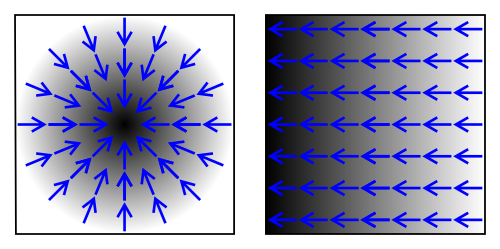
\includegraphics[width=0.7\textwidth]{images/Gradient}
      \caption{Quelle: Wikipedia: https://commons.wikimedia.org/wiki/File:Gradient2.svg}
\end{figure}


 \end{frame}


\begin{frame}
    \frametitle{Mehrdimensionale Differentialrechnung}
\framesubtitle{Differenzierbarkeit}
    \begin{block}{Gradient}

Sei   $f: U \to \mathbb{R}$ differenzierbare Funktion,  $a \in U$ und $v := \text{argmax}_{ ||h|| = 1 } \{ \partial_h f(a) \}$.
Dann gilt 
\begin{align*}
|| \nabla f(a) || v =  \nabla f(a) \; .
\end{align*} 
\end{block}

 \end{frame}

\begin{frame}
    \frametitle{Mehrdimensionale Differentialrechnung}
\framesubtitle{Differenzierbarkeit}
    \begin{block}{Beweis}
Mit der CSU Ungleichung folgt für beliebiges $h$ 
\begin{align*}
\partial_h f(a) = df(a) h = \langle \nabla f(a) , h \rangle = || \nabla f(a)||  \cdot ||h|| \cdot \cos(\varphi) 
\end{align*} 
wobei $\varphi$ den Innenwinkel zwischen $\nabla f(a)$ und $h$ bezeichnet. Für $||h|| = 1$ wird somit $\partial_h f(a) $ maximal, wenn $\varphi = 0$ und somit $h =  \nabla f(a)$ ist.
\end{block}

 \end{frame}

\end{document}

